% routing.tex
% Kapitel 4: Versuchsbeschreibung

\chapter{Versuchsbeschreibung}
\label{chapter:versuch}

Im Rahmen dieser Arbeit wurden die genannten Protokolle dahingehend angepasst, dass bei mehreren verfügbaren Wegen der Verkehr aufgeteilt wird, damit Teilnehmer mit einem begrenzten Energievorrat möglichst ausgeglichene Ladestände aufweisen. Dieses Kapitel widmet sich der eingesetzten Technik und deren Anpassung.

\section{Versuchsaufbau}
\label{chapter:versuch:aufbau}

\subsection{Eingesetze Technik}
\label{chapter:versuch:aufbau:technik}

Für die Simulation wurde folgende Software eingesetzt:

\begin{itemize}
\item Fedora Linux 26, 4.13.16-200.fc26.x86\_64
\item gcc-Version 7.2.1 20170915 (Red Hat 7.2.1-2) (GCC) 
\item Simulationssoftware OMNeT++, Version: 5.1
\item Framework Inetmanet-3.5
\end{itemize}

Bei \textit{OMNeT++} handelt es sich um ein Simulationssystem mit vielfältigen Möglichkeiten. Mittels dem Basis-Framework \textit{INET} lassen sich alle erdenklichen Protokolle, Szenarios oder Technologien aus dem Bereich Netzwerk in beliebiger Tiefe simulieren. Da \gls{manet} Protokolle leider nicht Bestandteil dessen sind, wurde es jedoch durch einen Fork \textit{Inetmanet} ersetzt. Letzteres stellt eine Erweiterung dar, in der diverse \gls{mesh} Protokolle zur Verfügung stehen. Das Framework besteht aus einer großen Sammlung von C++ Klassen, die sich durch konsequente Vererbung auszeichnen. Als IDE kommt die bei Entwicklern sehr populäre Eclipse-GUI zum Einsatz (Abbildung \ref{image:omnet:gui}) es kann jedoch auch mit einem Editor und dem C++ Compiler gearbeitet werden. Eine Simulation besteht in der Regel aus folgenden Elementen:

\begin{itemize}
\item Mindestens einer \textit{Network-Description-Datei (NED)}. Diese Dateien haben zwei Aufgaben: Zum einen dienen Sie als Bindeglied zu den C++ Klassen, in dem Sie Schnittstellen bedienen und selbst zur Verfügung stellen. Zum anderen werden sie für die Definition des Aufbaus von Simulationen genutzt. Abbildung \ref{listing:omnet:ned} zeigt ein einfaches Setup: Hier werden erst benötigte NEDs eingebunden, anschließend wird ein Netz mit dem Namen \textit{AODVCoreNetwork} und einem \textit{Objekt} vom Typ \textit{AODVRouter} definiert.
\item Mindestens einer \textit{Konfigurationsdatei (INI)}. Hier werden alle wichtigen Einstellungen für die Elemente der Network-Description vorgenommen. In Abbildung \ref{listing:omnet:ini} wird dem Objekt \textit{sender1} eine \textit{Ping-Anwendung} zugewiesen, die nach fünf Sekunden jede Sekunde eine Nachricht an das Objekt \textit{receiver1} sendet. Es besteht die Möglichkeit, mehrere Konfigurationsdateien durch Vererbung zu kombinieren.
\item Mindestens einer \textit{C++ Klasse}, die das eigentliche Verhalten der Objekte definiert. In der Regel wird in einer Klasse nur das ganz spezielle Verhalten des Objektes definiert, alle anderen Funktionen sind per Vererbung integriert.
\end{itemize}

Aus den benötigten Klassen wird mittels Compiler eine Bibliothek erzeugt, die für die Simulation genutzt wird. Hier gibt es wieder zwei Möglichkeiten:

\begin{figure}
  \centering
  \footnotesize
  \begin{lstlisting}[frame=single]
package powerrouting.simulations;
import powerrouting.node.aodv.AODVRouter;
import powerrouting.node.aodvpo.AODVPORouter;

network AODVCoreNetwork
{
    parameters:
        @display("bgb=1050,850");
    submodules:
        router32: AODVRouter {
            parameters:
                @display("i=device/pocketpc_s
                  ;r=,,#707070;p=400,250");
        }
    connections allowunconnected:
}
  \end{lstlisting}
  \caption{Auszug NED in OMNeT++}
  \label{listing:omnet:ned}
\end{figure}

\begin{itemize}
\item Eine grafische Oberfläche (Abbildung \ref{image:omnet:rungui}). Sie eignet sich besonders dann, wenn die Visualisierung der Prozesse im Vordergrund steht.
\item Die Ausführung per Kommandozeile. Dies bietet sich vor allem dann an, wenn man keine Interaktion wünscht. Es besteht die Möglichkeit automatisiert verschiedene Variablenbelegungen in mehreren Durchläufen mit verschiedenen Zufallszahlen zu testen. Zudem ergibt sich gegenüber der GUI ein Geschwindigkeitsvorteil.
\end{itemize}

\begin{figure}
  \centering
  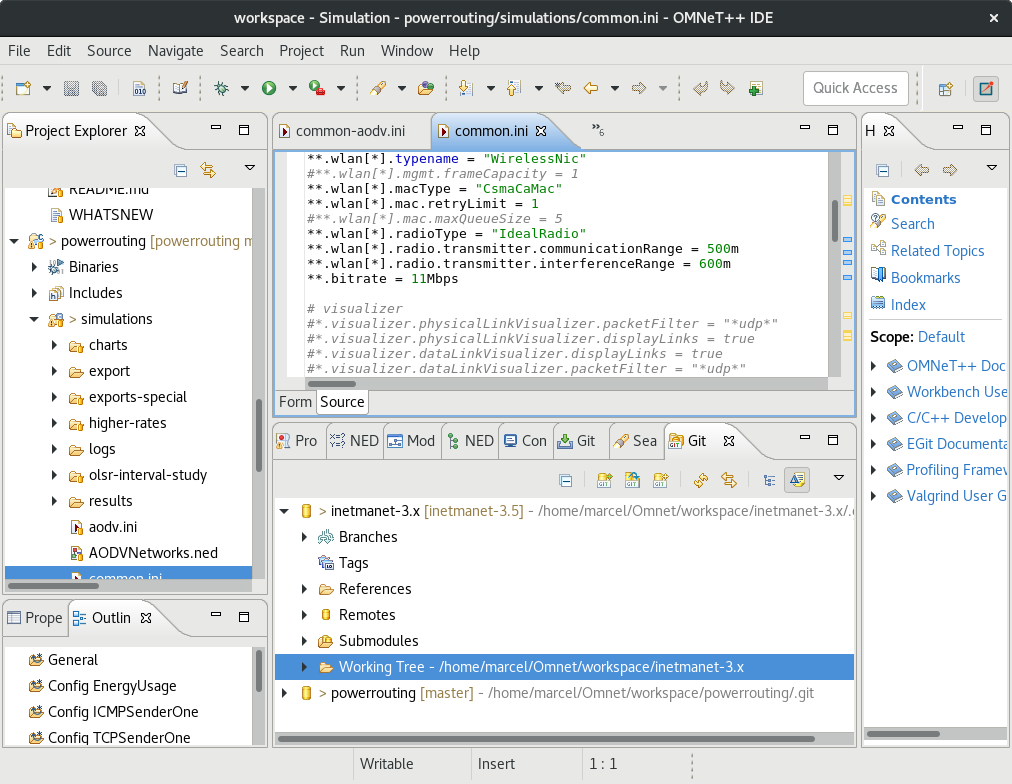
\includegraphics[scale=0.23]{bilder/gui1.png}
  \caption{IDE-GUI von OMNeT++}
  \label{image:omnet:gui}
\end{figure}

\begin{figure}
  \centering
  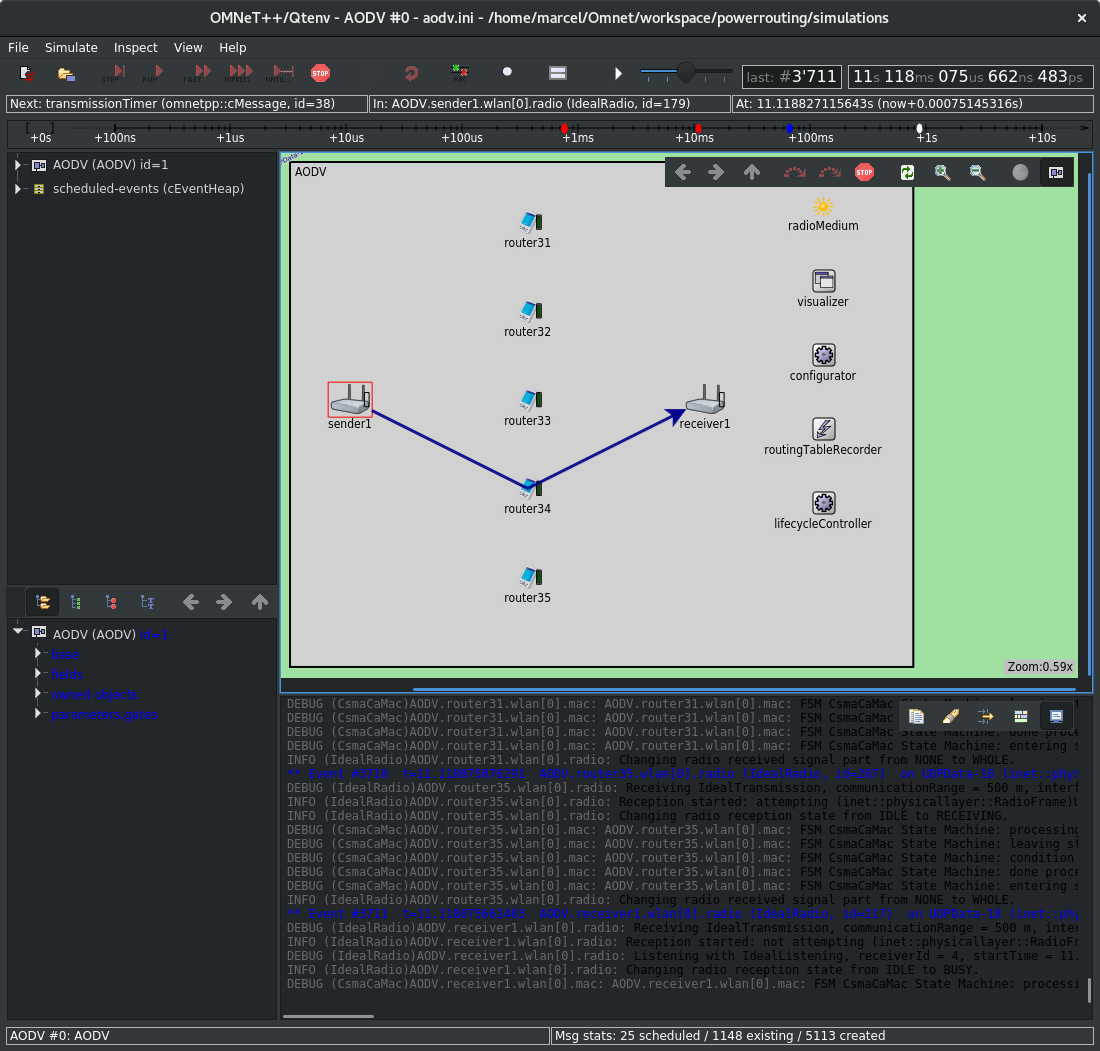
\includegraphics[scale=0.213]{bilder/gui2.png}
  \caption{Simulations-GUI von OMNeT++}
  \label{image:omnet:rungui}
\end{figure}

Die Simulationen erzeugen verschiedene Dateien, in denen alle Werte gemäß der Programmierung gespeichert sind. Des weiteren lassen sich die Nachrichten aller Objekte aufzeichnen. Eine tiefere Beschreibung der Möglichkeiten wird im nächsten Kapitel im Rahmen der Auswertung der Ergebnisse vorgenommen.\newline

Da die Anpassung von \gls{olsr} per Vererbung eine Änderung am Framework erforderlich gemacht hätte, wurden die für die Protokolle \gls{olsr} und \gls{aodv} benötigten Klassen komplett kopiert und in einen \textit{eigenen Namespace} überführt. Dort wurden die angepassten Versionen dann per Vererbung realisiert. Der gesamte Code, der im Rahmen dieser Arbeit erstellt wurde, steht unter der \gls{gpl} auf GitHub zur Verfügung.\footnote{https://github.com/marcelebbrecht/powerrouting} Da bei \gls{olsr} nur die einfachste Version genutzt wird, sind beide Verfahren nah an den jeweiligen \glspl{rfc} und vor allem für die angedachten Versuche hinreichend implementiert. Im Fall von \gls{aodv} scheint es in speziellen Fällen Probleme mit der \textit{loop avoidance} zu geben. Die Ursachen hierfür konnten aber nicht abschließend geklärt werden. Die Implementierung bestehen in der Regel aus folgenden Komponenten:

\begin{itemize}
\item Einer NED für die \textit{Router}, in der die Verwendung des jeweiligen \textit{Routingverfahrens} bestimmt und alle Eigenschaften und Funktionen eines \textit{Wireless Hosts} erbt.
\item Einer NED für das \textit{Protokoll}. Hier wird die Verbindung zu den \textit{C++ Klassen} hergestellt und es werden verschiedene \textit{Einstellungen} definiert.
\item Einer Sammlung aus \textit{C++ Klassen}, welche die Kontrollnachrichten und das Verhalten definieren.
\end{itemize}

\begin{figure}
  \centering
  \footnotesize
  \begin{lstlisting}[frame=single]
# ping sender one
**.sender1.numPingApps = 1
**.sender1.pingApp[0].destAddr = "receiver1(ipv4)"
**.sender1.pingApp[0].sendInterval = 1s
**.sender1.pingApp[0].startTime = 5s

  \end{lstlisting}
  \caption{Auszug INI in OMNeT++}
  \label{listing:omnet:ini}
\end{figure}

Leider sind die Protokolle nicht mit allen verfügbaren \textit{Radio}, \textit{MAC} und \textit{Interface-Typen} kompatibel umgesetzt. Es konnte jedoch eine Schnittmenge gefunden werden, um die Vergleichbarkeit sicherzustellen. Da nur das grundsätzliche Verhalten der Protokolle untersucht werden soll, wurde das verwendete Funkmodell möglichst einfach gewählt. Das Setup für die Simulationen lautet wie folgt:

\begin{itemize}
\item Als Schnittstellen-Typ wird \textit{WirelessNic} genutzt. Dieser stellt eine einfache \gls{wlan} Schnittstelle zur Verfügung.
\item Auf der \gls{maclayer} kommt \textit{CSMA/CA} zur Anwendung.
\item Als Radio-Typ wird \textit{IdealRadio} verwendet. Die Bitrate beträgt 11MBit/s, die Reichweite für die Übertragung 500m, die für Interferenzen 600m. Hierdurch können immer die jeweils direkten Nachbarn erreicht und gestört werden.
\item Zur Realisierung der endlichen Energiequelle und des Verbrauchers wurden die Klassen \textit{IdealEpEnergyStorage} und \textit{StateBasedEpEnergyConsumer} gewählt. Um die Bewertung der Ergebnisse zu vereinfachen, wurde der Energieverbrauch für alle Vorgänge, außer Senden, auf Null gesetzt. Bei den normalen Simulationen starten die Router mit derselben Ladung. Sie Sender und Empfänger verfügen jedoch über einen unbegrenzten Energievorrat.
\item Alle maßgeblichen Versuche wurden in \textit{100 Wiederholungen} mit verschiedenen Zufallszahlen durchgeführt, um eine hinreichende Signifikanz zu erreichen. Die Seeds wurden in der Konfiguration hinterlegt.
\item Die Simulationszeit beträgt in der Regel 180 Sekunden. Da bei kürzerer Laufzeit die Ergebnisse abweichen, wurde eine zusätzliche Auswertung für 60 Sekunden erzeugt um die Unterschiede transparent zu machen.
\item In den meisten Simulationen werden, nach einer \textit{Vorlaufzeit von 10 Sekunden}, \textit{UDP-Nachrichten} mit einem Abstand von circa \textit{50ms} verschickt.
\end{itemize}

\begin{figure}
  \centering
  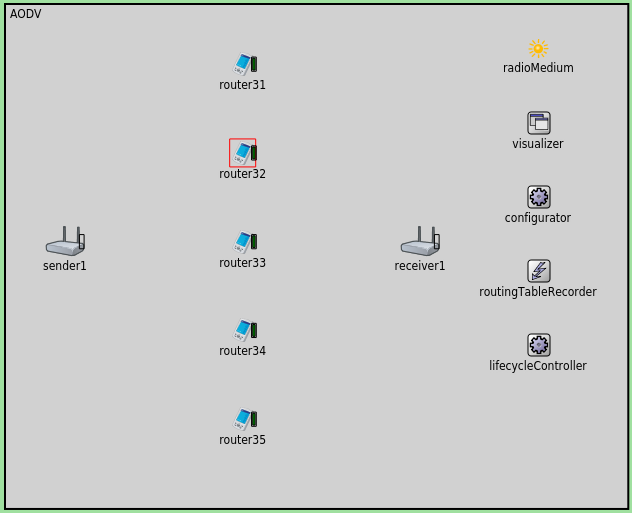
\includegraphics[scale=0.35]{bilder/aodv1.png}
  \caption{Single-Hop Testnetz}
  \label{image:omnet:aodv1}
\end{figure}

\subsection{Simulationsbeschreibung}
\label{chapter:versuch:aufbau:sim}

Für die verschiedenen Simulationen wurden folgende Topologien geschaffen:

\begin{itemize}
\item Ein Single-Hop Netz mit einem Sender, einem Empfänger und 5 Routern in der Mitte, die jeweils den Sender und Empfänger direkt erreichen können (Abbildung \ref{image:omnet:aodv1}).
\item Ein Multi-Hop Netz mit einem Sender, einem Empfänger, mehr Routern und einer geringeren Reichweite. Die Pakete müssen mindestens über 3 Router geleitet werden, bis sie das Ziel erreichen (Abbildung \ref{image:omnet:aodv2}).
\end{itemize}

\begin{figure}
  \centering
  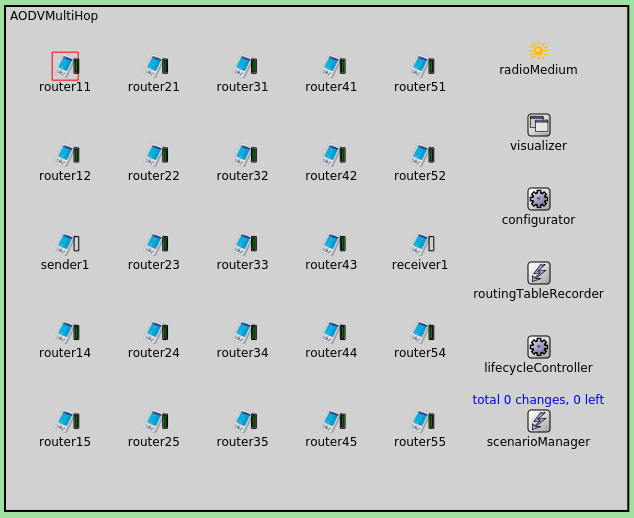
\includegraphics[scale=0.35]{bilder/aodv2.png}
  \caption{Multi-Hop Testnetz}
  \label{image:omnet:aodv2}
\end{figure}

Darüber hinaus gibt es weitere ergänzende Setups, auf welche in der Auswertung näher eingegangen wird: 

\begin{itemize}
\item Abweichende Ladung beim Start
\item Mischung aus angepasstem und normalem \gls{aodv}/\gls{olsr}
\item Eine ParameterStudy
\end{itemize}

\subsection{Neue Metrik}
\label{chapter:versuch:aufbau:metrik}

\begin{figure}
  \centering
  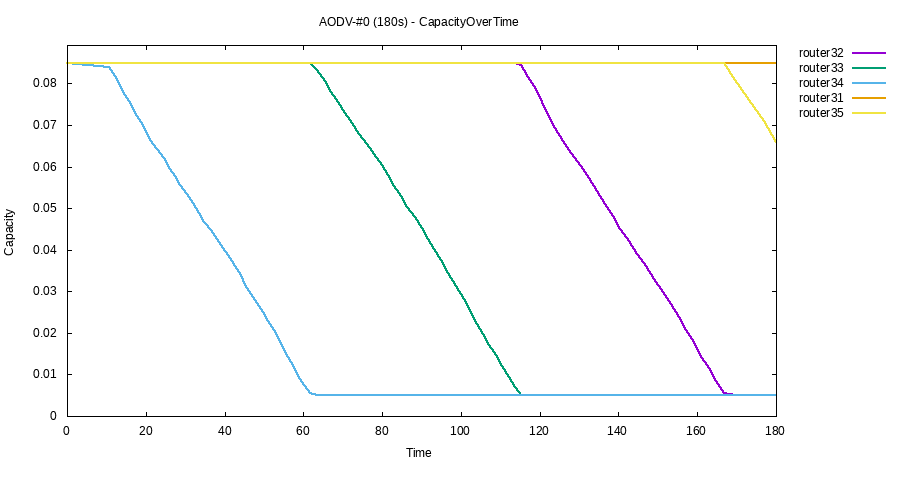
\includegraphics[scale=0.425]{bilder/aodv3.png}
  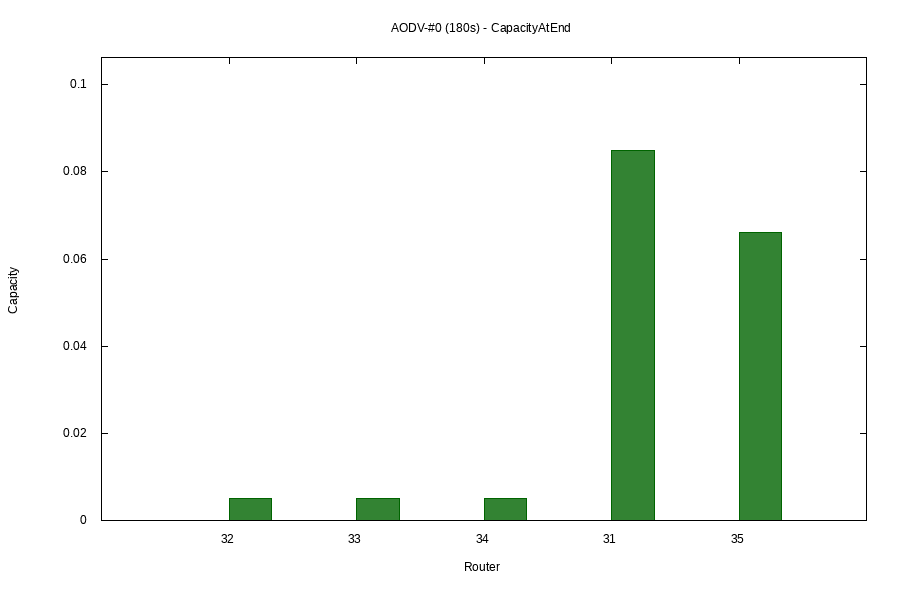
\includegraphics[scale=0.425]{bilder/aodv4.png}
  \caption{Energieverbrauch und -vorrat bei AODV nach 180 Sekunden}
  \label{image:omnet:aodv3}
\end{figure}

Die \glspl{rv} nutzen für die Bewertung der Routen den \textit{HopCount}, wobei bei \gls{olsr} auch die \textit{Willingness} in die Wahl der Gateways einbezogen wird. Um die Kompatibilität mit unangepassten Systemen beibehalten zu können, sollten diese Bewertungsmaßstäbe erhalten werden. Wie bereits in Kapitel \ref{chapter:routing} erwähnt, sollte also bei \gls{aodv} der \textit{HopCount}, bei \gls{olsr} die \textit{Willingness} manipuliert werden. Im Normalfall wird, nachdem einmal eine gültige Route ermittelt wurde, ein Pfad solange genutzt, bis ein Router auf dem Weg nicht mehr zur Verfügung steht. Wenn man davon ausgeht, dass dies nur durch Abschaltung aufgrund von unzureichender Ladung der Energieversorgung geschehen kann, dann wird in solch einem Netz eine Energieversorgung nach der anderen verbraucht (siehe Abbildungen \ref{image:omnet:aodv3}). Es ergibt sich also eine hohe Abweichung zwischen den Endständen. Da es das erklärte Ziel ist, die Weiterleitung von Paketen vom Stand der Energieversorgung der jeweiligen Router abhängig zu machen, muss eine neue Bewertungsmetrik definiert werden, die im weiteren als \textit{Energy fairness} bezeichnet wird. Je geringer die Abweichung der Energiestände am Ende der Simulation, desto \textit{fairer} ist die Verteilung. Die Metrik $M$ entspricht somit der Standardabweichung der Ladestände. Sei $n$ die Anzahl der Router, $C(i)$ die Restladung des jeweiligen Routers $i$ und $\bar{x} = \sum_{i=1}^{n} \frac{C(i)}{n}$ das arithmetische Mittel der Restladungen, dann gilt:
\begin{displaymath}
M = \sqrt{\sum_{i=1}^{n} \frac{(C(i)-\bar{x})^2}{n}} \\
\end{displaymath}
Je geringer dieser Wert ausfällt, desto ausgeglichener ist der Ladezustand und erfolgreicher die Anpassung. Allerdings muss auch berücksichtigt werden, dass Änderungen an den Routen zu Paketverlusten führen können, was bei häufigem Auftreten zu eklatanten Beeinträchtigungen führen kann. Um dies besser bewerten zu können, benötigen wird die \textit{Performance} $F$. Sei $L$ der durchschnittliche PacketLoss der Verbindungen im gesamten Netz und $c=10^{-10}$, dann gilt
\begin{displaymath}
F = ( 1 - ( L + c ) ) / ( M + c )
\end{displaymath}
Der Grad in dem eine Neuberechnung der Verbindungen stattfinden muss, hängt an ein paar spezifischen Einstellungen, welche in den nachfolgenden Abschnitten beschrieben und für die im Rahmen der Simulation mittels der \textit{ParameterStudy} optimale Werte ermittelt wurden.

\subsection{Anpassung AODV-PO (PowerOrientation)}
\label{chapter:versuch:aufbau:anpassungen-aodv}

Um den gewünschten Effekt zu erreichen, müssen die Router regelmäßig ihren Ladezustand überprüfen und dafür sorgen, dass die Routen angepasst werden. Durch das reaktive Design des Protokolls kommt es dabei aber zu kurzzeitigen Ausfällen, da erst eine neue Route ermittelt werden muss. Aus diesem Grund sollte die Anpassung nur nach einer signifikanten Änderung des Ladezustands eintreten. Diese Signifikanz wird im Weiteren als \textit{Trigger} $t$ bezeichnet und zwischen $0{,}1$ und $0{,}9$ gewählt. Sei $C(i)$ der relative Ladezustand des Hosts $i$ zwischen $0$ (leer) und $1$ (voll). Wenn \begin{displaymath}
(C(i) * 100) \mod (100t) = 0
\end{displaymath} 
gilt, wird eine Anpassung durchgeführt. So führt \zB $t=0{,}1$ zu einer Reaktion bei $100\%,90\%,80\%, ...$, also alle $10\%$. In diesem Fall wird ein \gls{rerr} erzeugt und nach dem bekannten Schema verschickt, damit eine Neubestimmung der Routen beginnt. Ferner soll es möglich sein den Grad der Veränderung anzupassen, was als \textit{Sensitivity} $s$ bezeichnet wird und zwischen $0{,}1$ und $10$ gewählt werden kann. Mit ihr kann bestimmt werden, wie stark der HopCount erhöht werden soll. Dieser Aufschlag wird als \textit{Penalty} $P$ bezeichnet. Im Normalfalls berechnet ein Router, der eine Verbindung per \gls{rrep} weitergibt den neuen HopCount $H_{neu}$ wie folgt aus dem ihm bekannten Wert $H_{alt}$:
\begin{displaymath}
H_{neu} = H_{alt} + 1
\end{displaymath}
In der angepassten Version wird in die Berechnung des neuen HopCounts $H'_{neu}$ die Penalty $P$ einbezogen, sofern der Router über einen begrenzten Energievorrat verfügt. Ferner kann in so einem Fall ein fester Aufschlag $B$ definiert werden, damit immer mit einer höheren Penalty agiert wird. Es gilt:
\begin{displaymath}
H'_{neu} = H_{alt} + 1 + P
\end{displaymath}
wobei die Penalty folgendermaßen berechnet wird:
\begin{displaymath}
P = \lceil\frac{s}{C_i} + B\rceil
\end{displaymath}
Bei $C(i) = 0{,}8$, $s = 2$ und $B=0$ ergibt sich also $P=\lceil\frac{2}{0{,}8} + 0\rceil = \lceil2{,}5\rceil = 3$ und somit $H'_{neu} = H_{alt} + 1 + 3 > H_{neu} = H_{alt} + 1$. Daraus folgt $H'_{neu} - H_{neu} = 3$, somit ist der Aufschlag durch den Router um 3 Hops höher. Er stellt sich also erheblich schlechter dar als er ist, damit andere Router \ggf andere Wege wählen sofern diese zur Verfügung stehen. Allerdings sollte $s$ mit Bedacht gewählt werden, da der Wert bei hohem $s$ und niedrigem $C(i)$ schnell steigt (er beträgt \zB für $s=10, C(i)=0.1$ bereits $100$) und die Anzahl maximaler Hops \textit{einer gesamten Route} auf 255 begrenzt ist. Daher sollte $s$ immer in Abhängigkeit der Größe des Netzes gewählt werden.\newline

Die Grundeinstellungen des Protokolls sind in OMNeT++ nach den Empfehlungen der RFC gesetzt und so belassen.

\subsection{Anpassung OLSR-PO (PowerOrientation)}
\label{chapter:versuch:aufbau:anpassungen-olsr}

Bei \gls{olsr} erfolgt die Anpassung auf ähnliche Art. Der Unterschied besteht allerdings in der Anwendung: Statt die Routen wie bei \gls{aodv} zu unterbrechen, wird die \textit{Willingness} der Hosts heruntergesetzt. Dies führt zwar zu einer gewissen Verzögerung bis die Routen geändert werden, allerdings entsteht keine Unterbrechung der Verbindungen. Stattdessen findet ein fließender Übergang statt. Daher ist \gls{olsr} durch geringeren \textit{PacketLoss} im Vorteil. Auch hier gibt es, aus den gleichen Gründen, einen Trigger $t$, der wie bei \gls{aodv} definiert ist. Der Grad der Veränderung, was erneut als \textit{Sensitivity} $s$ bezeichnet wird und zwischen $0{,}01$ und $0{,}99$ gewählt werden kann, bestimmt, wie stark die Willingness $W$ herabgesetzt wird. Auch hier erfolgt die Anpassung nur, wenn der Router über einen begrenzten Energievorrat verfügt. Ferner kann in so einem Fall ein fester Aufschlag $B$ definiert werden, damit immer mit einer höheren Penalty agiert wird. Es gilt:
\begin{displaymath}
W_{neu} = \lfloor\max(1,(7\cdot C(i)\cdot (1-s)-B))\rfloor
\end{displaymath}
Bei $C(i) = 0{,}8$, $s = 0{,}2$ und $B=0$ ergibt sich also $W_{neu} = \lfloor\max(1,(7\cdot 0{,}8\cdot (1-0{,}2)-0))\rfloor = \lfloor\max(1,4{,}48)\rfloor = 4$. Somit wird die Willingness auf den Wert 4 gesetzt. Hierdurch ist es möglich, dass Mitglieder der \glspl{1hnb}, die den Host als \gls{mpr} nutzen, auf einen anderen Host mit höherer Willingness als \gls{mpr} umstellen und somit der Verkehr über einen anderen Router geleitet wird, sofern dieser zur Verfügung steht. Auch hier sollte $s$ mit Bedacht gewählt werden, da bei hohem $s$ die Willingness sehr schnell sinkt.\newline

Die Grundeinstellungen des Protokolls wurden in OMNeT++ für die angepasste Version folgendermaßen gesetzt:
\begin{itemize}
\item \textbf{HELLO-Interval}: $2s$
\item \textbf{TC-Interval}: $5s$
\item \textbf{MID-Interval}: $5s$
\item \textbf{OLSR\_REFRESH-Interval}: $2s$
\end{itemize}

In der ursprünglichen Version wird statt dessen ein HELLO- und OLSR\_REFRESH-Interval von $0.5$ Sekunden genutzt. Dies erhöht zwar den Overhead, reduziert aber den Paketverlust durch ausgefallene Router drastisch.

